\documentclass{beamer}

\usepackage[utf8]{inputenc}
\usepackage{amsmath}
\usepackage{mathtools}
\DeclareMathOperator*{\argmax}{argmax} % thin space, limits underneath in displays
\mode<presentation>{
\usetheme{Madrid}
\usecolortheme{TOSU}
}

% Load biblatex package and .bib document
\usepackage{natbib}
\bibliographystyle{unsrtnat}

\AtBeginSection[]{
  \begin{frame}
  \vfill
  \centering
  \begin{beamercolorbox}[sep=8pt,center,shadow=true,rounded=true]{title}
    \usebeamerfont{title}\insertsectionhead\par%
  \end{beamercolorbox}
  \vfill
  \end{frame}
}

%Information to be included in the title page:
\title{An Introduction to Multi-label Learning}
\subtitle{(ML-KNN \& BP-MLL)}
\author{Bobby Lumpkin}
\date{}



\begin{document}

\frame{\titlepage}

\begin{frame}
\frametitle{Overview} % Table of contents slide, comment this block out to remove it
\tableofcontents % Throughout your presentation, if you choose to use \section{} and \subsection{} commands, these will automatically be printed on this slide as an overview of your presentation
\end{frame}

\section{Introduction to Multi-label Learning}

\subsection{Overview and Advantages}

\begin{frame}[t]{Multi-label Learning}
    \textbf{What is it?}
    \begin{itemize}
        \onslide<2->{
        \item[\rightarrow]
        Multi-label learning (mll) is a form of classification where each instance may be associated with more than one label.}
        
        \onslide<3->{
        \item[\rightarrow] 
        Plenty of tasks, such as text categorization, functional genomics, and supervised product recommendation fit naturally into the mll paradigm.}
        
        \begin{itemize}
            \onslide<4->{
            \item[*]
            \textbf{EX:} A news article discussing White House Covid press briefings might belong to each of the categories: ``News", ``Health" and ``Government".}
        \end{itemize}
    \end{itemize}
    
    \onslide<5->{
    \textbf{Why use novel approaches?}}
    \begin{itemize}
        \onslide<6->{
        \item[\rightarrow]
        Naive Approach: Train a sequence of independent binary classifiers (one per category)}
        
        \onslide<7->{
        \item[\rightarrow]
        Doesn't capitalize on the information in the correlations between the different labels of each instance.}
    \end{itemize}
\end{frame}

\begin{frame}[t]{Multi-label Paradigm: Definitions \& Notation}
    \begin{itemize}    
        \item 
        Let $\chi$ denote the domain of instances and $\mathcal{Y} = \{1,...,Q\}$ be the finite set of labels. 
        
        \item
        Given $x \in \chi$ and its associated $Y \subseteq \mathcal{Y}$, let $\vec{y}_x$ be the category vector for $x$ such that (for all $\ell \in \mathcal{Y}$) $\vec{y}_x(\ell) = 1$ if $\ell \in Y$. Otherwise, $\vec{y}_x(\ell) = 0$. 
    \end{itemize}
\end{frame}

\section{ML-KNN Approach}

\subsection{Model Outline}

\begin{frame}[t]
\frametitle{ML-KNN Algorithm: More Notation}
    \textbf{Notation:}
    \begin{itemize}
        \onslide<2->{
        \item
        Let $N(x)$ denote the set of $K$ nearest neighbors of $x$, identified in the training set.}
        
        \onslide<3->{
        \item
        Let $\vec{C}_x(\ell) = \sum_{a \in N(x)} \vec{y}_a(\ell)$ ($\ell \in \mathcal{Y}$) define a membership counting vector.}
        
        \onslide<4->{
        \item
        Let $H_0^\ell$ denote the event that test instance $t$ does not have a label $\ell$ and let $H_1^\ell$ denote the event that it does have label $\ell$.}
        
        \onslide<5->{
        \item
        Let $E_j^\ell$ ($j \in \{1,...,K\})$ denote the event that, among the $K$ nearest neighbors of $t$, there are exactly $j$ instances which have label $\ell$.}
    \end{itemize}
\end{frame}

\begin{frame}[t]{ML-KNN Algorithm: Overall Approach}
    \small
    \textbf{Overall Approach:}
    This ML-KNN algorithm takes a parametric, Bayesian approach towards estimating the Bayes Optimal Classifier. As with the single-label algorithm, it does this using the K nearest neighbors of an instance. Namely...
    
    \begin{itemize}
        \onslide<2->{
        \item 
        Given a test instance, $t$, $\vec{Y}_t$ is determined using the MAP estimate:}
        
        \onslide<3->{
        \begin{align*}
            \vec{y}_t(\ell) &= \argmax_{b \in \{0, 1\}} \mathbb{P}\left(\textrm{H}_b^\ell | E_{\vec{C}_t(\ell)}^\ell\right), \textrm{\hspace{0.3cm}}\ell \in \mathcal{Y} \\
            &= \argmax_{b \in \{0,1\}} \frac{\mathbb{P}\left(\textrm{H}_b^\ell\right) \cdot \mathbb{P}\left(E_{\vec{C}_{t(\ell)}}^\ell | \textrm{H}_b^\ell\right)}{\mathbb{P}\left(E_{\vec{C}_t(\ell)}^\ell \right)} \\
            &= \argmax_{b \in \{0, 1\}}\mathbb{P}\left(\textrm{H}_b^\ell\right) \cdot \mathbb{P}\left(E_{\vec{C}_{t(\ell)}}^\ell | \textrm{H}_b^\ell\right)
        \end{align*}}
        
        \onslide<4->{
        \item
        Where we take a Bayesian approach towards estimating the prior probabilities, $\mathbb{P}\left(\textrm{H}_b^\ell\right)$, and conditional probabilities, $\mathbb{P}\left(E_{\vec{C}_{t(\ell)}}^\ell | \textrm{H}_b^\ell\right)$.}
        \normalsize
    \end{itemize}
\end{frame}

\begin{frame}[t]{ML-KNN Algorithm: Overall Approach continued...}
    \textbf{Definition:} Let $\vec{\textrm{r}}_t$ denote the real-valued vector with $\ell^{th}$ component: 
    
    $$
        \vec{\textrm{r}}_t(\ell) \coloneqq \mathbb{P}\left(\textrm{H}_1^\ell\right).
    $$
    \begin{itemize}
        \onslide<2->{
        \item[\Rightarrow] 
        Thus, given training data, $\mathcal{X}$, and a test instance, $t$, we wish to compute $[\vec{y}_t(\ell), \vec{r}_t(\ell)]$.}
    \end{itemize}
\end{frame}

\subsection{Computing Model Probabilities}

\begin{frame}[t]{ML-KNN Algorithm: Computing the Prior Probabilities, $\widehat{\mathbb{P}(\textrm{H}_b^{\ell})}$}
    \small
    We model $\mathbb{P}(\textrm{H}_1^\ell)$ with a $\textrm{Beta}(s,s)$ prior and $\textrm{Binomial}(m, \textrm{ }\mathbb{P}(\textrm{H}_1^\ell))$ likelihood. (When $s = 1$, $\textrm{Beta}(s, s)$ reduces to the uniform distribution on $[0, 1]$.)
    
    \begin{itemize}
        \onslide<2->{
        \item[\Rightarrow] 
        The posterior distribution for $\mathbb{P}(\textrm{H}_1^\ell)$ is:
        
        $$
            \textrm{Beta}\left(s + \sum_{i = 1}^m \vec{y}_{x_i}(\ell), \textrm{ }s + m - \sum_{i = 1}^m \vec{y}_{x_i}(\ell)\right).
        $$}
        
        \onslide<3->{
        \item[\Rightarrow]
        We will estimate $\mathbb{P}(\textrm{H}_1^\ell)$ with the expectation of it's posterior Beta distribution:
        
        $$
            \widehat{\mathbb{P}(\textrm{H}_1^\ell)} \coloneqq \frac{s + \sum_{i = 1}^m \vec{y}_{x_i}(\ell)}{2s + m}
        $$
        
        where $m$ is the number of training instances.}
        
        \onslide<4->{
        \item[\Rightarrow]
        We estimate $\widehat{\mathbb{P}(\textrm{H}_0^\ell)} \coloneqq 1 - \widehat{\mathbb{P}(\textrm{H}_1^\ell)}$.}
    \end{itemize}
\end{frame}

\begin{frame}[t]{ML-KNN Algorithm: Computing the Conditional Probabilities, $\widehat{\mathbb{P}(E_j^\ell | \textrm{H}_b^\ell)}$}
    \small
    \textbf{Definition:} 
    \begin{itemize}
    \onslide<2->{
        \item[(i)]
        Let $c$ be a vector of length $K + 1$, where $c(j) =$ the number of training instances where $\vec{C}_{x_i}(\ell) = j$ when $\vec{y}_{x_i}(\ell) = 1$.}
        
        \onslide<3->{
        \item[(ii)]
        Similarly, let $c^{\prime}$ be a vector of length $K + 1$, where $c(j) =$ the number of training instances where $\vec{C}_{x_i}(\ell) = j$ when $\vec{y}_{x_i}(\ell) = 0$.}
    \end{itemize}
    
    \textbf{Model:}
    \begin{itemize}
        \onslide<4->{
        \item[*]
        We let $\overrightarrow{\mathbb{P}(E_j^\ell | \textrm{H}_1^\ell)} = (\mathbb{P}(E_1^\ell | \textrm{H}_1^\ell),...,\mathbb{P}(E_K^\ell | \textrm{H}_1^\ell))$ (analogously for $\overrightarrow{\mathbb{P}(E_j^\ell | \textrm{H}_0^\ell)}$)}
        
        \onslide<5->{
        \item[*]
        We give $\overrightarrow{\mathbb{P}(E_j^\ell | \textrm{H}_1^\ell)}$ (and $\overrightarrow{\mathbb{P}(E_j^\ell | \textrm{H}_0^\ell)}$) a $\textrm{Dirichlet}(K + 1, (s,...,s))$ prior distribution.}
        
        \onslide<6->{
        \item[*] 
        We use a $\textrm{Multinomial}(K+1, (\frac{c(0)}{m_1},...,\frac{c(K)}{m_1}))$ likelihood, where $m_1 = \sum_{i = 1}^m \vec{y}_{x_i}(\ell)$ (analogously for $\overrightarrow{\mathbb{P}(E_j^\ell | \textrm{H}_0^\ell)}$).}
        
    \end{itemize}
\end{frame}

\begin{frame}[t]{ML-KNN Algorithm: Computing the Conditional Probabilities, $\widehat{\mathbb{P}(E_j^\ell | \textrm{H}_b^\ell)}$ continued...}
    \small
    \begin{itemize}
        \item[\Rightarrow]
        The posterior distribution for $\overrightarrow{\mathbb{P}(E_j^\ell | H_1^\ell)}$ is
        
        $$
            \textrm{Dirichlet}\bigg(K + 1, \Big(s + c(0), ... , s + c(K)\Big)\bigg)
        $$
        
        (and analogously for $\overrightarrow{\mathbb{P}(E_j^\ell | H_0^\ell}$).
        
        \onslide<2->{
        \item[\Rightarrow]
        Given $j \in \{0,...,K\}$, we estimate $\mathbb{P}(E_j^\ell | H_1^\ell)$ and $\mathbb{P}(E_j^\ell | H_0^\ell)$ with the expectations of their posterior distributions:}
        
        \onslide<3->{
        \begin{align*}
            \mathbb{P}(E_j^\ell | H_1^\ell) &\coloneqq \frac{(s + c(j))}{((K + 1)s + \sum_{n = 0}^K c(n))} \\
            \mathbb{P}(E_j^\ell | H_0^\ell) &\coloneqq \frac{(s + c^{\prime}(j))}{((K + 1)s + \sum_{n = 0}^K c^{\prime}(n))}
        \end{align*}}
    \end{itemize}
\end{frame}

\begin{frame}[t]{Computing $\vec{y}_t$ and $\vec{r}_t$}
    \small
    Using our previous derivation:
    
    $$
        \widehat{\vec{y}_t(\ell)} \coloneqq \argmax_{b \in \{0, 1\}} \left[\widehat{\mathbb{P}(H_b^\ell)} \cdot \widehat{\mathbb{P}(E_{\vec{C}_T(\ell)}^\ell | H_b^\ell)} \right]
    $$
    
    \onslide<2->{
    \begin{center}
        AND
    \end{center}}
    
    \onslide<3->{
    \begin{align*}
        \widehat{\vec{r}_t(\ell)} &\coloneqq \frac{\widehat{\mathbb{P}(H_1^\ell)} \cdot \widehat{\mathbb{P}(E_{\vec{C}_T(\ell)}^\ell | H_1^\ell)}}{\sum_{b \in \{0, 1\}}\left[\mathbb{P}(H_b^\ell) \cdot \mathbb{P}(E_{\vec{C}_t(\ell)}^\ell | H_b^\ell)\right]} \\
        &= \frac{\widehat{\mathbb{P}(H_1^\ell)} \cdot \widehat{\mathbb{P}(E_{\vec{C}_T(\ell)}^\ell | H_1^\ell)}}{\mathbb{P}(E_{\vec{C}_t(\ell)}^\ell)}
    \end{align*}}
    
    \onslide<4->{
    \textbf{NOTE:} The larger the value for $s$, the less importance assigned to the training data: As $s \rightarrow \infty$, $\vec{r}_t(\ell) \rightarrow \frac{1}{2}$.}
\end{frame}

\subsection{Implementation (in scikit-multilearn)}

\begin{frame}[t]{Scikit-multilearn Implementation}
    \textbf{\underline{Scikit-multilearn:}}
    \small
    \begin{itemize}
        \item
        The \textbf{``scikit-learn"} module is a free and widely used software machine learning library for Python, including many popular regression, classification and unsupervised learning algorithms.
        
        \onslide<2->{
        \item
        The \textbf{``scikit-multilearn"} module is a library for multi-label classification that is built on top of the scikit-learn ecosystem.}
    \end{itemize}
    
    \vspace{0.15cm}
    \normalsize
    \onslide<3->{
    \textbf{\underline{ML-KNN Classification in scikit-multilearn:}}}
    \begin{columns}
    \small
        \column{0.5\textwidth}
        \begin{itemize}
        \onslide<4->{
            \item[\rightarrow] 
            MLkNN() from the scikit-multilearn module can be used to instantiate a ML-KNN object.}
            
            \onslide<5->{
            \item[\rightarrow]
            ``MLkNN" class methods like ``fit()" and ``predict()" mirror those for standard scikit-learn objects.}
        \end{itemize}
        \column{0.5\textwidth}
        \onslide<4->{
        \begin{figure}[htp]
            \centering
            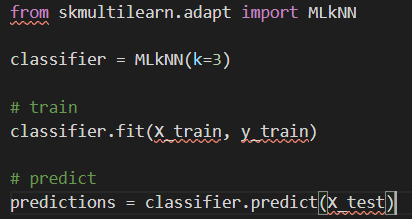
\includegraphics[width = 5.35cm]{mlknn_example_code.PNG}
        \end{figure}}
    \end{columns}
\end{frame}

\section{BP-MLL Approach}

\subsection{Feed-forward Neural Networks}

\begin{frame}[t]{A Brief History}
    \scriptsize
    \begin{columns}
        \column{0.5\textwidth}
        \begin{itemize}
            \onslide<2->{
            \item 
            Inspired by biological nervous systems, neural networks date back to the first half of the 20th century with works such as those by McCulloch and Pitts, which could model simple logical operations.}
            
            \onslide<3->{
            \item
            Since most subsequent work in the following two decades centered around single layer networks, the power of neural networks was restricted to linearly separable problems.} \onslide<4->{This excluded the possibility of learning even simple functions like XOR, which required a second layer.}
            
            \onslide<5->{
            \item
            In the early 1980s, research on neural networks resurged largely due to successful learning algorithms for multi-layer neural networks and are used today for various tasks such as computer vision, associative memory, representation learning, NLP, etc..}
        \end{itemize}
        
        \column{0.5\textwidth}
        \onslide<2->{
        \begin{figure}[htp]
            \centering
            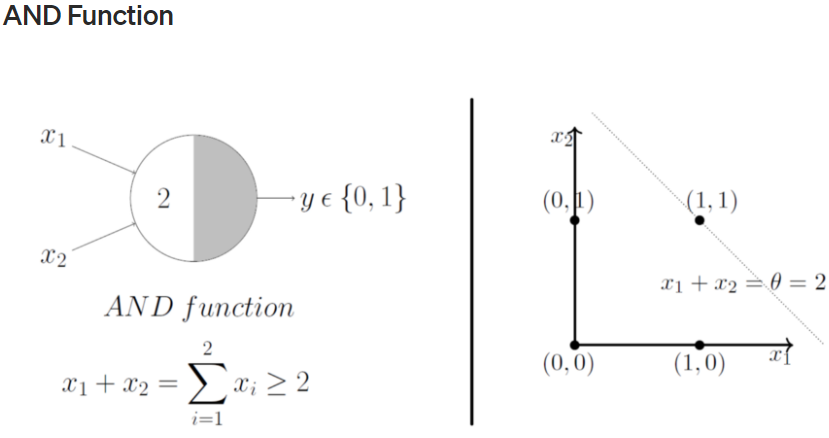
\includegraphics[width = 4cm]{McCullochPitts_and_gate.PNG}
        \end{figure}}
        
        \onslide<4->{
        \begin{figure}[htp]
            \centering
            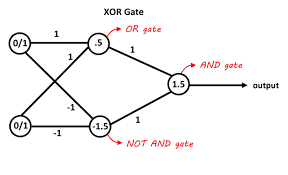
\includegraphics[width = 3.5cm]{Multi_layer_McCullochPitts_XOR.png}
        \end{figure}}
        
        \onslide<5->{
        \begin{figure}[htp]
            \centering
            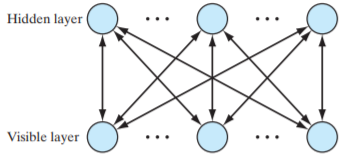
\includegraphics[width = 3.5cm]{restricted_Boltzmann_machine_diagram.PNG}
        \end{figure}}
    \end{columns}
\end{frame}

\begin{frame}[t]{Introduction to Feed-forward Networks: Perceptron Model}
    The perceptron model (the building block for feed-forward networks) can be viewed as a connected, directed, loop-free graph like the one below.
    
    \small
    \begin{columns}
        \column{0.5\textwidth}
        \begin{itemize}
            \onslide<2->{
            \item 
            Neurons in the first layer represent components of the input vectors.}
            
            \onslide<3->{
            \item
            The output of the neuron in the next layer is determined by applying a non-linear ``activation function" to a linear combination of the input components, plus a bias.}
            
            \onslide<4->{
            \item
            Rosenblatt's Perceptron model uses a step function non-linearity, but other common activation functions include the sigmoid function ($\sigma()$), tanh$()$, ReLU, Leaky ReLU, softmax, etc..}
        \end{itemize}
        
        \column{0.5\textwidth}
        \begin{figure}[htp]
            \centering
            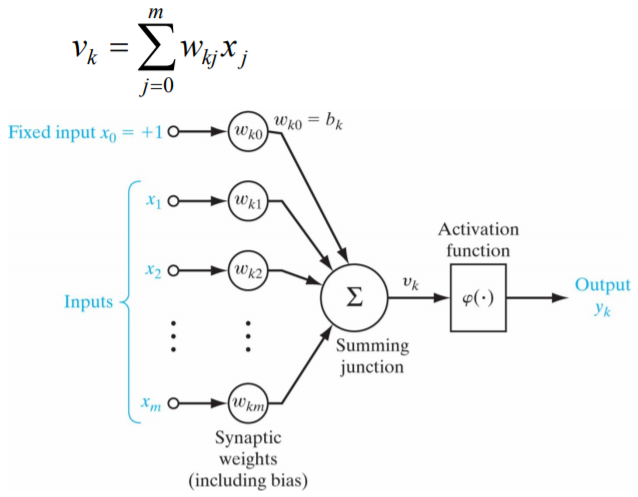
\includegraphics[width = 6cm]{Perceptron_Model_Diagram_Haykin.PNG}
        \end{figure}
    \end{columns}
\end{frame}

\begin{frame}[t]{Multilayer Networks \& Training}
    \begin{itemize}
        \item 
        Adding additional layers and units (like in the network pictured below) significantly expands the class of discrimination problems a network can learn.
        
        \onslide<2->{
        \item
        ``Online" training involves evaluating an instance, and updating weights using gradient descent.}
        
        \onslide<3->{
        \item
        For multi-label learning with $Q$ instances, networks will have $Q$ output layers, each with a tanh() activation.}
    \end{itemize}
    
    \begin{figure}[htp]
        \centering
        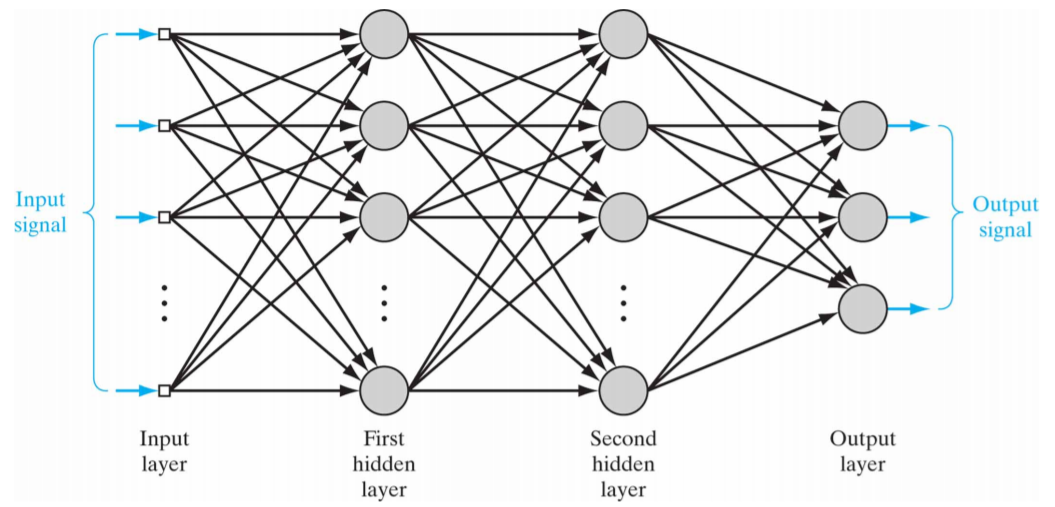
\includegraphics[width = 6.5cm]{multilayer_network_Haykin.PNG}
    \end{figure}
\end{frame}

\subsection{Neural Network Loss Functions \& Training for MLL}

\begin{frame}[t]{Designing a Cost Function}
    \footnotesize
    As for standard networks, BP-MLL uses gradient descent \& back propagation for learning. The novelty of the approach is in the design of the cost function. \\
    \onslide<2->{
    \textbf{\underline{Naive Approach (``BasicBP"):}}
    \begin{itemize}
        \item
        Standard MSE: 
        
        $$
            E = \sum_{i = 1}^m E_i = \sum_{i = 1}^m \sum_{j = 1}^q(c_j^i - d_j^i)^2
        $$
        
        where $c_j^i = c_j(x_i)$ is the output of the network on $x_i$ on the $j^{th}$ class.
    \end{itemize}}
    
    \onslide<3->{
    \textbf{\underline{Novel Approach (``BP-MLL"):}}}
    \begin{itemize}
        \onslide<3->{
        \item 
        BP-MLL Cost function:
        
        $$
            E = \sum_{i = 1}^m E_i = \sum_{i = 1}^m \frac{1}{|Y_i| |\overline{Y}_i|} \sum_{(k,l) \in Y_i \times \overline{Y}_i} \exp(-(c_k^i - c_l^i))
        $$
        so that the $i^{th}$ error term is severely penalized if $c_k^i$ is much smaller than $c_l^i$. \\}
        
        \onslide<4->{
        \item
        Back-propagation for training is derived just as in the standard (MSE) case (details omitted here, but can be found in Zhang and Zhou's paper).}
    \end{itemize}
\end{frame}


\subsection{Implementation (in TensorFlow/Keras)}

\begin{frame}[t]{Deep Learning APIs in Python: TensorFlow/Keras}
    \textbf{\underline{TensorFlow:}} an open source python library for numerical computation and large-scale machine learning, created by the Google Brain team.
    \begin{itemize}
        \item[\rightarrow] 
        One of the most widely used APIs for deep learning, along with PyTorch and Keras.
        
        \item[\rightarrow]
        Later versions of TensorFlow began incorporating the Keras API, since users found its high-level design to be simpler.
    \end{itemize}
    
    \begin{figure}[htp]
        \centering
        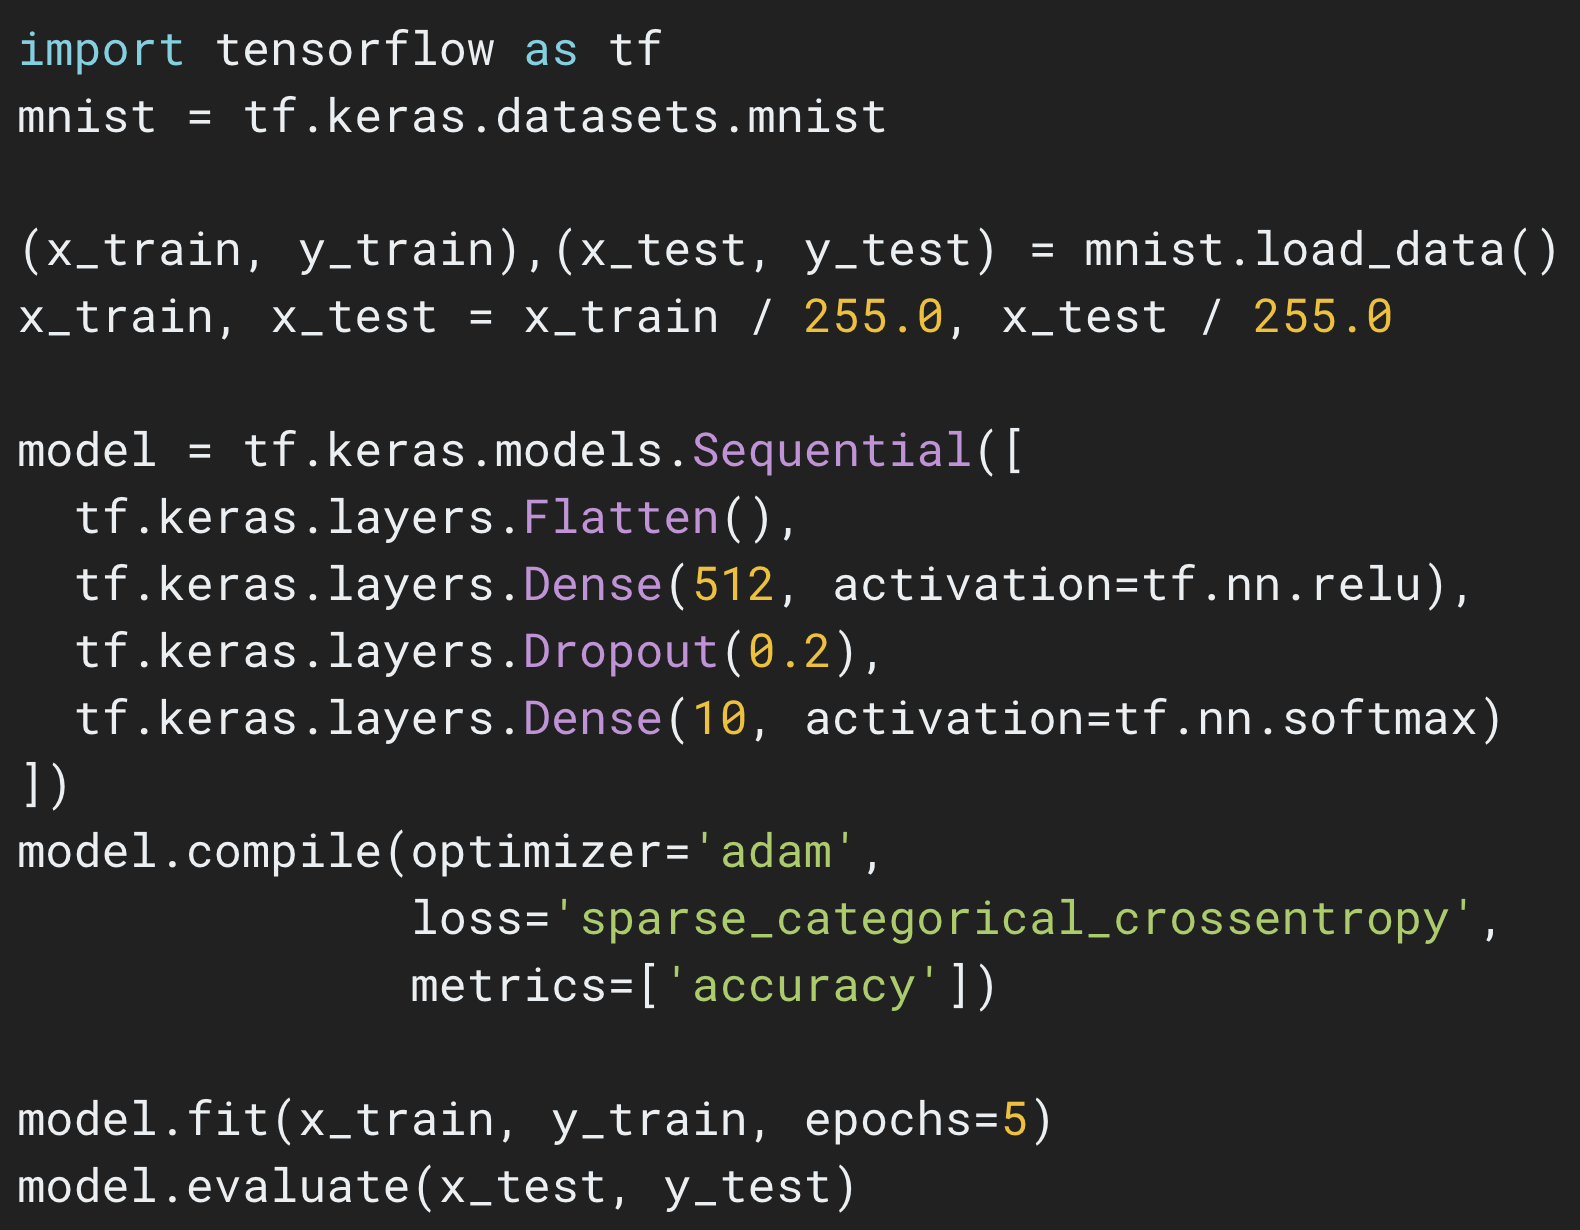
\includegraphics[width = 5.5cm]{basic_tensorflow_keras_code.png}
    \end{figure}
\end{frame}

\begin{frame}[t]{TensorFlow Implementation of BP-MLL}
    \textbf{\underline{BP-MLL in TensorFlow:}}
    \begin{itemize}
        \item[\rightarrow]
        Data Scientist, Lukas Huwald, published an implementation of the bp-mll cost function for the TensorFlow API as part of the module ``bpmll".
        
        \item[\rightarrow]
        After installation, the bp-mll loss function can be utilized just as any other TensorFlow loss function.
    \end{itemize}
    
    \begin{figure}[htp]
        \centering
        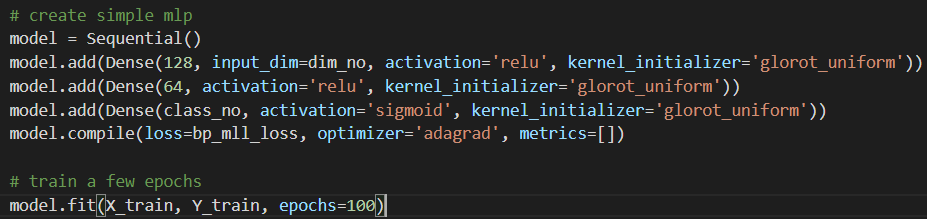
\includegraphics[width = 10.5cm]{bpmll_example_code.PNG}
    \end{figure}
\end{frame}

\begin{frame}[t]{Potential Cause for Caution}
    \scriptsize
    Both Zhang and Zhou's original paper as well as \cite{bp_mll_revisited} provide reasons for potential caution when considering application of the BP-MLL loss function:
    
    \begin{itemize}
    \onslide<2->{
        \item[\rightarrow] 
        \textbf{Computational Inefficiency:} Because the BP-MLL loss function involves pairwise comparisons, obtaining error terms is more expensive than utilizing cross-entropy or MSE loss.} \onslide<3->{This scales poorly with the number of labels, and can lead to significantly larger training times.}
        
        \onslide<4->{
        \item[\rightarrow]
        \textbf{Objective Function Surface:} The surface for the BP-MLL loss has plateaus in which gradient descent can be very slow in comparison with the cross-entropy, for example (\cite{bp_mll_revisited}).
        
        \begin{figure}[htp]
            \centering
            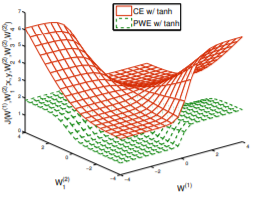
\includegraphics[width = 4cm]{Nam_et_al_2014_bpmll_plateau.PNG}
        \end{figure}}
        
        \onslide<5->{
        \item[\rightarrow]
        \textbf{Generalization:} When compared against a ``standard" feed forward network with dropout regularization, adaptive learning rates and ReLU hidden layer activations, the test-set performance of BP-MLL is inferior on benchmark datasets for large scale text categorization (\cite{bp_mll_revisited}).}
    \end{itemize}
\end{frame}

\begin{frame}[t]{References (Original Method Papers)}
    \nocite{mlknn}
    \nocite{bpmll}
    \bibliography{mll_osu}
\end{frame}

\end{document}
